% Intended LaTeX compiler: pdflatex
\documentclass[11pt]{article}
\usepackage[utf8]{inputenc}
\usepackage[T1]{fontenc}
\usepackage{graphicx}
\usepackage{grffile}
\usepackage{longtable}
\usepackage{wrapfig}
\usepackage{rotating}
\usepackage[normalem]{ulem}
\usepackage{amsmath}
\usepackage{textcomp}
\usepackage{amssymb}
\usepackage{capt-of}
\usepackage{hyperref}
\author{Miguel Angel Escalante Serrato}
\date{13.08.21}
\title{\#Verificado19s}
\hypersetup{
 pdfauthor={Miguel Angel Escalante Serrato},
 pdftitle={\#Verificado19s},
 pdfkeywords={},
 pdfsubject={},
 pdfcreator={Emacs 27.2 (Org mode 9.4.4)}, 
 pdflang={Spanish}}
\begin{document}

\maketitle

\section{Introducción}
\label{sec:org4463394}
\(\int\)\textsubscript{0}\textsuperscript{1}e\textsuperscript{-x\textsuperscript{2}}
\subsection{Sismo en CDMX}
\label{sec:org0e81e26}
\begin{itemize}
\item Sismo con 7.1 grados de magnitud escala de Richter.
\item Daños generalizados en la CDMX.
\item Área con alta densidad poblacional.
\end{itemize}
\subsection{Tecnología en respuesta}
\label{sec:org29d2579}
\begin{itemize}
\item Buena parte de la población urbana tiene un teléfono celular.
\item Independientemente de la conectividad, son cámaras de bolsillo.
\item Se generó mucha información al instante:
\begin{itemize}
\item Videos de edificios en movimiento.
\item Cadenas de Whatsapp.
\item Videos de edificios colapsando.
\end{itemize}
\end{itemize}
\subsection{Desinformación}
\label{sec:org0c3555b}
El proncipal problema con la información que la población compartió en el momento fue que no tenía orden.
\begin{itemize}
\item Falta de especificidad
\item No contiene ubicaciones
\item Fragmento de información
\end{itemize}
\subsection{Desinformación}
\label{sec:orgb8c99e0}
Las publicaciones en redes sociales
\begin{itemize}
\item Información Falsa
\item Conenido Tendencioso
\item Información Vieja
\end{itemize}
\subsection{Respuesta Ciudadana}
\label{sec:org9cc57ec}
\begin{center}
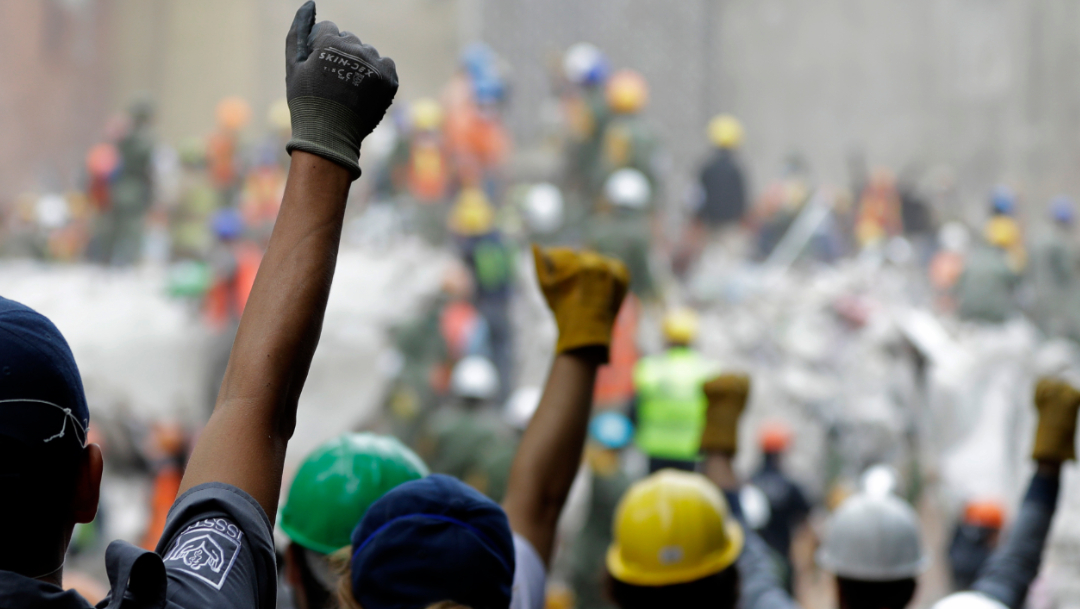
\includegraphics[width=.9\linewidth]{./img/sismoimg.jpeg}
\end{center}


\section{Verificado 19s}
\label{sec:orgc43bfee}
\subsection{¿Qué fue \#Verificado19s?}
\label{sec:org249b599}
Verificado19s fue un colectivo que activó la respuesta a las peticiones de ayuda por parte de buena parte de la población. Llegamos a ser más de 300 voluntarios racabando información y redirigiendo ayuda.
Tuve el privilegio de tomar el liderazgo de todo lo relacionado a la tecnología del colectivo

\subsection{Mapa Original}
\label{sec:org4316144}
\begin{itemize}
\item Sergio Beltrán genera un mapa con información que a él le parece pertinente
\item Comparte el mapa con un grupo cercano
\item Tiene que atender una emergencia
\item El mapa se vuelve viral.
\end{itemize}
\subsection{Mapa Congelado}
\label{sec:org5c4e658}
Dada la cantidad de personas accediendo al mapa, y editándolo el mapa dejó de funcionar, aunque seguía siendo accesible para visualizar. Las personas aún podían ver la información pero no podían agregar más.

\subsection{20 de septiembre}
\label{sec:org31d30f6}

Ante la sobrecarga del mapa, los voluntarios comenazaron a guardar la información que se iba reportando al colectivo en papel y lápiz.
\section{Objetivo}
\label{sec:org449f233}

Encontrar una manera de:
\begin{itemize}
\item Capturar reportes ciudadanos
\item Unificar ingesta de información
\item Unificar diversas fuentes
\item Limpiar información
\item Verificar información
\end{itemize}

\section{Soución}
\label{sec:org592a213}
\subsection{Ingesta}
\label{sec:org4421080}
\begin{itemize}
\item Google Forms
\item Diversas fuentes de información
\end{itemize}
\subsection{Procesamiento}
\label{sec:org176dfe8}
\begin{itemize}
\item Limpieza de datos personales
\item Mecanismo de actualización
\end{itemize}
\subsection{Inteligencia}
\label{sec:org49808ed}
\begin{itemize}
\item Capa de verificación
\item Ubicación automática en con la dirección
\item Coordinación logística
\end{itemize}
\subsection{Visualización}
\label{sec:orgcab734b}
\begin{itemize}
\item La capa final fue MyMaps en un principio
\item Movimos el mapa a Google Crisis Map
\end{itemize}
\subsection{Crisis Map}
\label{sec:org9207960}
\begin{itemize}
\item Decisión muy costosa.
\item Mapa mucho más robusto.
\item Ya no disponible.
\end{itemize}


\section{Caso Haití 2010}
\label{sec:orge8d2530}

\subsection{Ushahidi}
\label{sec:orgcae66d8}
Nace de las elecciones de 2008 en Nairobi, Kenia.
Plataforma para mapeo masivo de información, recabando datos de diversas fuentes:
\begin{itemize}
\item SMS
\item Twitter
\end{itemize}
\subsection{Ushahidi - Haití}
\label{sec:org982e453}
Se requirieron diversas herramientas extras para el manejo de la crísis humanitaria en 2010.
\begin{itemize}
\item SMS
\item Equipo Verificadores
\item Humanitarian OpenStreetMap
\end{itemize}
\subsection{Humanitarian OpenStreetMape}
\label{sec:org0f25ac8}
\begin{itemize}
\item Es un sistema de crowsourcing para mapeo de zonas que están en algun riesgo.
\item Se hace a manera de Wikipedia un manejo de proyecto y necesidades de mapeo que luego publican a cualquier voluntario para que pueda suplira.
\end{itemize}
\subsection{Humanitarian OpenStreetMap -Haití}
\label{sec:orgc0f0fbd}
\begin{itemize}
\item El principal problema que se encontraron durante la respuesta al sismo del 2010, fue que no existían mapas lo suficientemente confiables.
\item Para ello desplegaron una serie de peticiones sobre la zona y conforme fueron pasando las semanas, se fueron mejorando los mapas.
\end{itemize}


\section{¿Qué tal si ?}
\label{sec:orge2dbffa}

\subsection{Aplicación móbil}
\label{sec:org4f8caa6}
Una aplicación que permita el reporte sencillo de incidentes con capacidad de hacer peticiones de ayuda, materiales o voluntarios.
\subsection{Asignación inteligente de recursos.}
\label{sec:org618c3d6}
Un sistema que pueda capturar las peticiones de los sitios de desastre, buscarlos automáticamente en una base de datos donde se registre la oferta de materiales y voluntarios, podría ayudar a mejorar considerablemente la asignación de recursos a los diferentes sitios.

\section{Conclusiones}
\label{sec:org7fbb452}
\end{document}